\cleardoublepage
\appendix

%TODO Are the tables necessary for the point you want to make?
\chapter{Logging practice in software engineering}
Providing a guide for software engineers and developers to implement a suitable logging implementation in their software systems has to prove to be a vital tool in both industrial use and progress of academia \cite{Rong2018a}. Guoping Rong et al.~made a study to review these logging practices published papers to improve the performance and efficiency of logging implementation. From his study he made selection criteria to include (as in \Cref{tbl:CH1_RongIncSelectionCriteria}) and exclude (as in \Cref{tbl:CH1_RongExlSelectionCriteria}) academic papers about logging practices \cite{Rong2018a,Rong2018}.\par The Rong's selection criteria obtained numerous research papers of logging practices applied in the industry by either creating a new logging mechanism or optimising existing logging mechanisms. By reviewing 41 identified papers he found that many practitioners and researchers recognise the importance of logging practice in software engineering. There is a lack of guidance to provide software engineers or developers to create or improve their efficient logging mechanisms \cite{Rong2018a,Zhu2015}. 

\begin{table}[!htb]
	\centering
	\small
	\caption[G. Rong's inclusion selection criteria]
	{\textit{G. Rong's inclusion selection criteria \cite{Rong2018a}}}
	\label{tbl:CH1_RongIncSelectionCriteria}
	\begin{tabularx}{\textwidth}{|c|X|}
		\hline \textbf{Identification} & \textbf{Criteria} \\
		\hline I1. & Publications that investigate the methodology for logging practice. \\
		\hline I2. & Publications that investigate the tools, frameworks, systems which support logging practice. \\
		\hline I3. & Publications that propose a standard for logging practice.\\
		\hline I4. & Publications that are peer-reviewed (conference paper, journal article). \\
		\hline I5. & Publications that are primary studies on logging practice. \\
		\hline
	\end{tabularx}
\end{table}

\begin{table}[!htb]
	\centering
	\small
	\caption[G. Rong's exclusion selection criteria]
	{\textit{G. Rong's exclusion selection criteria \cite{Rong2018a}}}
	\label{tbl:CH1_RongExlSelectionCriteria}
	\begin{tabularx}{\textwidth}{|c|X|}
		\hline \textbf{Identification} & \textbf{Criteria} \\
		\hline E1. & Publications that investigate log analysis. \\
		\hline E2. & Publications that investigate the usage of logs. \\
		\hline E3. & Publications that investigate the technologies on logging user behaviours. \\
		\hline E4. & Publications that are not written in English. \\
		\hline E5. & Additionally, short papers, demo or industry publications are excluded. \\
		\hline
	\end{tabularx}
\end{table}

\clearpage

In \Cref{fig:PushblisedPapers} shows the distribution of the 41 published papers obtained for Rong's research relating to logging practices. Event logging has an increasingly important role in modern software systems, therefore the research focus on logging practices in software engineering have been on a rise between 1990 and 2017.

\begin{figure}[!htb] % An h :here, t: top, b: bottom.
	\centering % cent the figure
	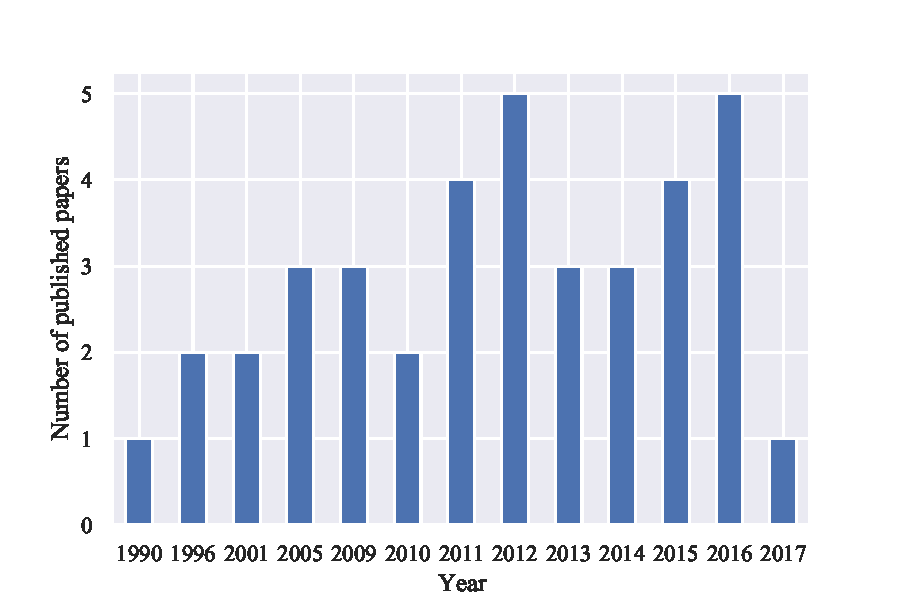
\includegraphics[width=0.9\textwidth]{Chapter1/Ronga2018.pdf}
	\caption[The distribution of the papers’ published years]
	{\textit{The distribution of the papers’ published years \cite{Rong2018a}}} \label{fig:PushblisedPapers}
\end{figure} 
